In Part \ref{part:related_work}, we have seen the various facets of password-based authentication problems. However, a few central problems remain understudied and deserve further attention: has user education been successful in the past decade and in which ways? How severe is the threat of password reuse and are there ways to detect it and to mitigate risks? 

The next chapters shed light on these aspects of the problem space of usable password security. 

\chapter[Mental Models of Password Strength]{Mental Models of \\
	Password Strength}\label{chap:pasdjo}

This chapter reports on findings published at OzCHI 2017 \cite{Seitz2017PASDJO}. The insights and data are put into context and extended with additional analyses. 

\section{Background and Context}
% Assumption: Users don't know how to create strong passwords
Users create passwords on a regular basis. As discussed in Chapter \ref{chap:rw:user_perspective}, previous research indicates that users most commonly resort to weaker passwords that are easy to remember. In case the account value is higher, however, it is suspected that users invest more effort into creating a stronger password. Password meters are helpful in this context \cite{Egelman2013DoesMyPasswordGoUpToEleven}. Yet, even these stronger passwords are often ineffective against sophisticated guessing attacks, so it stands to reason that users have a faulty mental model of what makes a strong password. This has been a commonly accepted assumption \ar but it oversimplifies the state of affairs. 

% perceptions and mental models change over time. 
First, mental models change over time -- both on a micro- and a macro-scale. At micro-scale, it is evident that the first passwords are chosen in teenage years and without much care for security \cite{VonZezschwitz2013SurvivalShortest}. Over time, users are exposed to password advice and educational nudges: popular news portals regularly publish new articles that report on data breaches or warn about risky online behavior. This and incidents in one's own social network \cite{Stobert2014PasswordLifeCycle} raise awareness about the topic and can spark plans to behave differently in the future. Moreover, registering with multiple services increases the likelihood of facing different password policies and password meters which nudges users to reflect on their password choice. Potentially they might also alter their mental models if feedback and policy instructions are well-designed \cite{Shay2015SpoonfulOfSugar, Ur2017DataDrivenPWMeter}.

% education seems to have paid off.
Zooming out to the macro level, efforts to educate users may have already paid off. In the early days of research in Usable Security, often the user was seen as the ``weakest link'' in a secure system \cite{Adams1997MakingPWsSecureAndUsable, Sasse2005UsableSecurityPosition}. When Florêncio and Herley conducted their large-scale study in 2006/2007, they saw relatively low-entropy passwords, but higher-value accounts were a bit better protected. However, in 2015 Ur \etal found that users' mental models had become better which allowed them to create stronger and memorable passwords \cite{Ur2015PWCreationLab}. A year later, they presented an in-depth analysis of the perceptions of password strength \cite{Ur2016PerceptionsPassword}. They found that for the most part, participants in their online-study were capable of identifying the factors that add to password strength. Shay \etal already used ``perceived strength'' as a proxy metric \cite{Shay2015SpoonfulOfSugar}, and it seems this is a better approach than one might think. For a few notable exceptions, though, certain password characteristics fooled participants. Ur \etal argue that errors in mental models about strength arise from false understandings of attackers. Consequently, it would be necessary to shift education from password strength towards attackers, because users already have a fairly accurate understanding of strength. 

%TODO maybe add a third argument here (perceptions might be the)
%or: Florencio / finite effort stating that users are smarter than we might think
Florêncio \etal put forward a formal model as to why users behave insecurely. Their central argument is that it is inevitable to choose weak passwords for some accounts and that users are well aware of their behavior. Yet, if users have a faulty understanding of password strength then the selection process is biased. In the case of users also showing the overconfidence bias, where people are subjectively more confident in their abilities and judgments than the objective accuracy of the judgments \cite{Simonson1989ChoiceBasedOnReasons}, this could indeed lead to considerable risks.  %TODO go on. 

% summary: perceptions are still understudied 
In summary, having a clear mental model of what makes for a strong password is essential to make the decision whether to use one or not. While there are initial results, the perceptions of these factors is still understudied to this point.

\subsection{Research Objectives}
In this project, I wanted to investigate the origin of weak passwords. I challenged the folk model that users behave insecurely due to their lack of knowledge (as proposed by \ar). If users are able to identify weak and strong passwords, it is fair to assume they can select appropriately strong passwords depending on the situation. With this knowledge, we can rethink password feedback. As pointed out above, current password meters and verbal feedback might be ineffective because if the majority of users is aware of the strength of their password. Instead, feedback could be framed around re-use or attack models. Solidifying evidence from related work with a novel study approach was a fruitful step towards making a holistic design recommendation regarding the feedback aspect of password support systems. 

%\begin{itemize}
%	\item find more evidence of password misconceptions
%	\item educate users at the same time? --> problematic because we didn't really focus on it and left it to the users to figure out how it works.
%\end{itemize}

\subsubsection{Research Questions}
The specific research questions for this project were as follows:
\begin{itemize}
\item[RQ1] How well can users identify weak and strong passwords?
\item[RQ2] What types of password topologies lead to the most errors?
\end{itemize}


%\section{Related Work}

\section{Approach: PASDJO - The Password Game}
To evaluate (in)accuracies in mental models about password strength, I chose to have users rate passwords similarly to the study task in Ur \etal's study \cite{Ur2016PerceptionsPassword}. In their presentation at CHI 2016, they challenged the audience which sparked the idea of making a game out of this task. To open the game to a large audience, I decided to implement it as a web-application that runs in any web browser on various platform. 

\begin{figure}
	\centering
	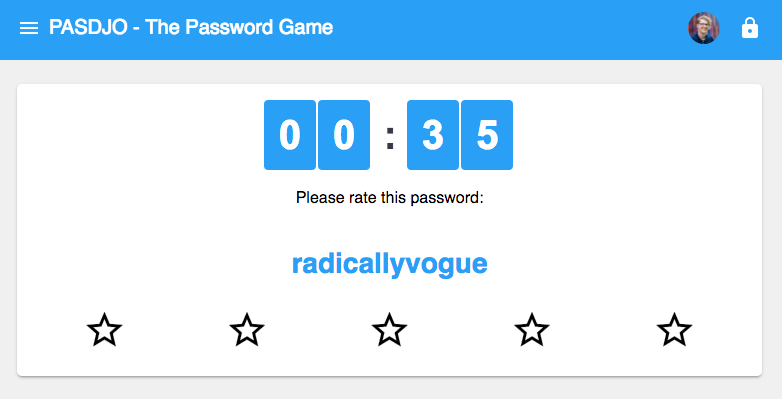
\includegraphics[width=0.75\textwidth]{pasdjo/radicallyvogue}
	\caption{\label{fig:pasdjo:radicallyvogue}}
\end{figure}

\subsection{Game Mechanics and Design Elements}
The game is relatively simple: Players judge how strong or weak a given password is. They receive points by accurately estimating the strength of a given password on a scale from 1 (weak) to 5 (strong). The game follows similar design strategies for the password topologies as the Ur \etal's online study, but passwords are either randomly taken from large dictionaries or generated on the fly. To induce intuitive estimations, a time-limit is enforced while a ``highscore'' acts as incentive to estimate as accurately as possible. To reach higher scores, one has to judge as many passwords as possible in 60 seconds. 

\subsubsection{Scoring and Metrics}
A crucial point of the game is how the passwords are rated objectively. Here, we rely on the zxcvbn library\footnote{\url{https://github.com/dropbox/zxcvbn}} (described in detail in Section \ref{sec:rw:pw_strength_metrics}) because it is highly reliable and straightforward to use on a web page. It also comes with a number of word lists that are helpful to implement different scenarios, respectively conditions. Beside the guess-number metric, zxcvbn also scores passwords on a scale from zero (weak) to four (strong). We translate this scale to one star (weak) to five stars (strong) in the game. 

For a correct estimation -- ``correct'' in the sense that zxcvbn comes to the same strength estimation -- a player is awarded 100 points. The difference between the user's rating and the zxcvbn score is  the \textbf{\textit{deviation}} ($D$). A player's rating can deviate by at most four stars, e.g. if they rate a five-star password with a score of one and vice versa. In that case, the player should not get any points, but in all other cases, the player is still awarded fewer points. For each integral deviation in either direction there is a penalty of 25 minus-points (maximum of 100 points, at most 4 errors, which leads to $100 / 4 = 25$). The points of the estimations are summed up and build the \textbf{\textit{achieved}} score ($A$). As an overall accuracy measure, at the end of the game we calculate the ratio of achieved and possible points and display it as percentage ($P$). 

The game thus implements the following scoring function, where $U$ is the user's estimation on a scale from 1 to 5, $Z$ is the zxcvbn score on the same scale, and $n$ is the number of passwords a user has rated within the time limit. 

\noindent The scoring function takes an array of user ratings and zxcvbn scores for $n$ passwords and returns a vector consisting of the achieved points $A$ and accuracy metric $P$.
\[
f([(U|Z)_1, ..., (U|Z)_n]) = (A|P)
\]

\noindent For each estimation the deviation from the zxcvbn score is calculated.
\[
D_k = U_k - Z_k\\
\]

\noindent The total achieved points are the sum of the achieved points per round. Each round takes the 25 point penalty into account. If $|D_k|=0$, the player gets the full 100 points per round.
\[
A = \sum_{k}^{n} 100 - (|D_k|*25) \\
\]
\noindent Finally, the accuracy is the fraction of achieved and possible points. 
\[
P = \frac{A}{n * 100}\\
\]

The score and accuracy are displayed to the users once the game is finished, see Figure \ref{fig:pasdjo:feedbackscreen}.

\begin{figure}
	\centering
	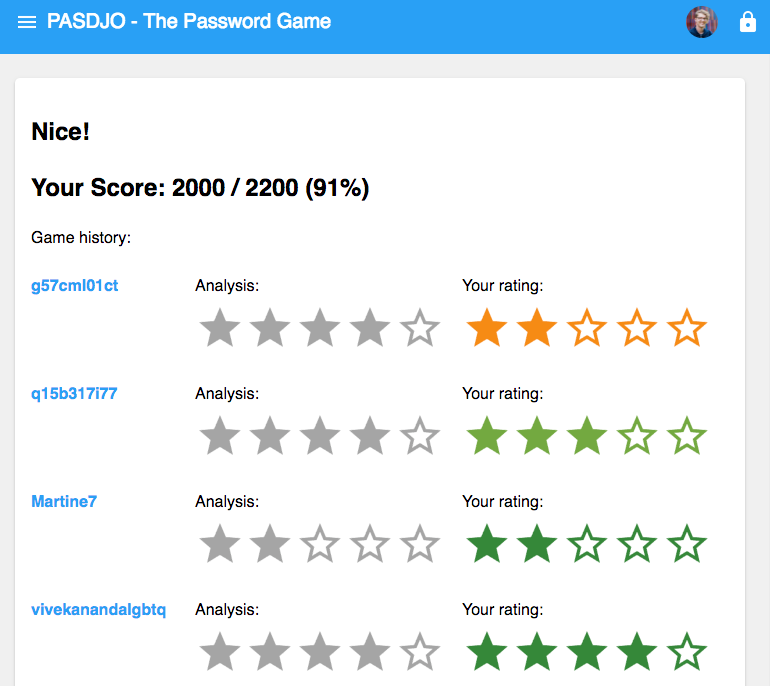
\includegraphics[width=0.75\textwidth]{pasdjo/feedbackscreen}
	\caption{\label{fig:pasdjo:feedbackscreen}}
\end{figure}

\subsubsection{Persuasive Design Elements}
discuss: 

low barrier to play the game: easy to understand, only takes one minute (persuasive weapon: commitment, small favors)
motivation: you might learn something or you can evaluate if your knowledge is correct (persuasive weapon: authority zxcvbn tells you what's correct) and discuss with other people. you can challenge your assumptions. 

we could also argue with Fogg Behavior model. 

%TODO Persuasive patterns (re Nicolas' comment at OzCHI)

\subsection{Password Generation and Study Conditions}
\makeatletter
PASDJO initially had four different password types that act as levels of the independent variable: Common passwords, mangled passwords, passphrases, and random passwords. During gameplay, the condition for the next password was selected at random. The following paragraphs depict the conditions in detail. 


\textbf{Common passwords: } We take the word lists that come with the zxcvbn library. One of these lists contains 47023 leaked passwords ordered by frequency, from which we randomly pick one for this condition. The data stems from breaches of user databases at RockYou, Yahoo and Xato \cite{Wheeler2016zxcvbn}. All passwords are lower-case and can be considered weak, because they are usually amongst the first attempts in a guessing attack \cite{Ur2015MeasuringRealWorldAccuracies} unless the adversary launches a targeted attack where personal information plays a more important role. Zxcvbn rates the top 1000 passwords with a score of 1 (e.g. ``12345'', ``password'', ``monkey''), and the remaining passwords are scored with two stars (e.g. ``iloveyou2'', ``skywalker'', ``apollo13''). It is worth noting that many of these passwords would not be accepted anymore by websites as common policies demand at least 8 characters (see Chapter \ref{chap:policies-reuse}), which RockYou and Xato did not enforce at the time. %TODO the last remark could go somewhere else. 


\textbf{Mangled passwords: } For the mangled password condition, we take the same list of the top 47023 passwords, but we algorithmically substitute certain characters. The substitutions look like ``leet''  / ``l33t'' speak, which is a typical way to try to increase password strength \cite{Das2014TangledWeb, Mazurek2013Measuring}. For instance, an ``a'' is replaced by an ``\@'', or an ``s'' is substituted with the dollar sign ``\$''. Also, random characters are transformed to uppercase. To allow recognizing the original word, we only mangle up to 30\% of the characters of the password. Since we only use substitutions that zxcvbn recognizes, mangled passwords mostly receive a score of two. However, in rare occasions, they occupy the full range, i.e., ``p@ssw0rd'' (1), ``b0n3he@d'' (2), ``fireFI9hter'' (3), ``123qaz456w\$x'' (4), ``123Q@z4s6w\$x'' (5). 


\textbf{Random passwords: } We implemented a simple string generation algorithm to create random passwords. They are lowercase alphanumeric passwords containing letters from the German alphabet, i.e. [a-z0-9äöü]. Zxcvbn consistently gives them a score of four, which makes them easy to rate. In a real-world attack they can only be brute-forced \cite{Florencio2014AdministratorsGuide, Wheeler2016zxcvbn}.


\textbf{Passphrases: } We combine two entries from the English Wikipedia index to create a passphrase (also shipped with zxcvbn). The words were required to be between 4 and 11 characters long. This restriction leads to a dictionary size of 27202 entries. Thus, there are $27202^2 \approx 10^9$ possible combinations, which is unpredictable enough to withstand online guessing attacks. This is reflected by the rather high scores: zxcvbn gives passphrases mostly a score of three or four, e.g. ``armedtamils'' (3), ``boostedeuros'' (4). If the words appear in other dictionaries, e.g. the ``TV subtitles'' word list, they are more likely to result in a score of three. However, for a user it is not straight-forward to tell whether a passphrase scores three or four points, which makes this condition harder to get right. 

\vspace*{2ex}
For the remainder of the chapter we refer to these four condition as ``Common'', ``Mangled'', ``Random'', and ``Passphrase''.


\subsection{Benefits and Shortcomings of the Game-based Approach}
Since the game was deployed publicly, the method can be denoted as an unsupervised in-the-wild study. This approach has certain benefits and shortcomings as discussed in the following. 

\subsubsection{Benefits}
\textbf{Easy collection of multiple data points per user} The game can be played over and over. A survey could also be taken multiple times, but most of the time this is not desirable. If the study is done via MTurk this would mean that people would be paid each time which drives costs.

\vspace*{1ex}
\noindent\textbf{Possibility to provide feedback} After the game, the players can review their ratings and find out how they performed. In a study, implementing such a feedback loop is much more complicated and often impossible with current survey tools. Hence, a debriefing step is required, but it's difficult to tailor it to the individual participant.

\vspace*{1ex}
\noindent\textbf{Randomization and password space} Ur \etal's study was designed well in that it tested a wide range of password characteristics and there were multiple options per condition. However, the options were predefined by the researchers and limited in that sense. In our case, we can pick passwords from much larger word-lists at random and use algorithms to randomly adjust certain characteristics. This allows for higher internal validity of the data collection.

\vspace*{1ex}
\noindent\textbf{Intrinsic Motivation} The game is 

\subsubsection{Drawbacks}

Lack of demographics

playing on multiple devices is hard to trace

disclaimers are somewhat hidden as a trade off of lowering the barrier to play the game

\subsection{Implementation}
polymer firebase webpage PWA 
UX considerations: load quickly, run offline and large data transfer (mobile first paradigm), disclaimers
\section{Log Analysis}

\subsection{Sample}

December 2016 until March 2017
two important events: Open Lab Day of our research group and student orientation day at LMU central
Thus, it is likely that most players were students or in academia. 

What data did we throw out and why? how much of the dataset is that?

\subsection{Results}

%TODO consider running another test a year afterwards.


\section{Discussion}

\section{Limitations}
\begin{itemize}
	\item were already addressed in new versions of the game. 
	\item used as an activity at Google	
\end{itemize}


\section{Summary}
\begin{itemize}
	\item users performed better than anticipated
	\item misconceptions mainly involve passphrases and mangled passwords
	\item the game was updated after the first results were in and is still deployed. Google even uses it internally. 
	\item the source code is available on GitHub.
\end{itemize}

\section{Improvements in Revisions}
see slides from talk
updated scoring
more evenly distributed scores and conditions
updated passphrase generation algorithm (not just two words, but randomly 2 or 3, random punctuation)
leaderboard (game design element)

\subsection{Future Work}
Better onboarding
Challenges
Player Profiles 
adding the game to password management software

